\documentclass[conference]{IEEEtran}
\IEEEoverridecommandlockouts
\usepackage{amsmath,amssymb}
\usepackage{graphicx}
\usepackage{booktabs}
\usepackage{cite}
\usepackage[caption=false,font=footnotesize]{subfig}
\usepackage{microtype}
\graphicspath{{figures/}}

\title{Dynamic Cage Reconstruction and Curriculum Reinforcement Learning for Continuous Tracking of Moving Targets}
\author{
\IEEEauthorblockN{Jiarun Shi and Xiaodong Feng*}
\IEEEauthorblockA{
School of Information Science and Technology\\
Beijing University of Chemical Technology, Beijing, China\\
\{2023030094, 2002500022\}@buct.edu.cn}
\thanks{*Corresponding author: Xiaodong Feng.}
}

\begin{document}
\maketitle

\begin{abstract}
Continuous tracking of a moving object is difficult when visual latency, intermittent depth measurements, and manipulator dynamics jointly create a following error that can move the object beyond the robot's observation and effective control range. The end-effector reference should therefore reflect not only the latest measured center but also prior experience about poses that are favorable for capture and unfavorable for escape. This paper presents a dynamic Cage reconstruction and control framework for a UR5e manipulator with an eye-in-hand RGB-D camera. Offline, motion-consistent Cage candidates are evaluated through repeated rigid-body simulations using the actual internal geometry of a U-shaped gripper, and the selection experience is summarized as a compact arc prior. Online, five visual observations initialize a position--velocity--acceleration estimate; subsequent Kalman filtering, local spline fitting, and motion-plane estimation reconstruct a six-dimensional Cage reference without access to future samples. A bounded Jacobian controller provides deterministic large-error approach, while a curriculum-trained proximal policy optimization policy performs high-rate local joint-velocity correction. The simulation includes depth noise, pixel loss, and whole-frame dropout rather than ideal state feedback. The resulting modular pipeline combines the interpretability and reach of model-based control with the responsiveness of learned local control, improving the stability and agility of continuous moving-object tracking.
\end{abstract}

\begin{IEEEkeywords}
Dynamic caging, eye-in-hand vision, moving-target tracking, proximal policy optimization, visual motion estimation.
\end{IEEEkeywords}

\section{Introduction}

Continuous observation and manipulation of a moving object are fundamental to interception, in-motion handling, and close-range human--robot interaction. Unlike static reaching, the object continues to move while an image is acquired, processed, and converted into a robot command. A controller that reacts only to the latest measured center therefore accumulates delay-dependent tracking error. With an eye-in-hand camera, the same error can move the object outside both the observation field and the effective control range.

Moving-target visual servoing provides the closest background. Ito and Shibata compensated target motion in an image-based eye-in-hand controller for a planar hand--eye robot \cite{ito2009}. Shahriari \emph{et al.} treated target-induced feature motion as a disturbance, combining depth and motion observation with focus-of-expansion information \cite{shahriari2013}. These works demonstrate that motion estimation can reduce visual following delay, but their objectives are image-feature regulation rather than construction and tracking of a three-dimensional, motion-aware Cage reference.

In this work, a Cage denotes an open end-effector pose selected to be favorable for capture and unfavorable for target escape; it is not a sealed enclosure. Candidate quality is evaluated against the actual U-shaped internal gripper geometry. The previously considered construction obtained by rotating the fingers by $\pm30^{\circ}$ to form a swept three-dimensional Cap is explicitly excluded. Offline dynamics simulation acquires Cage-selection experience, and online reconstruction reuses this experience without repeating the expensive candidate search.

The control problem spans two regimes. Differential Jacobian control produces an interpretable descent direction and rapidly handles a large pose discrepancy, whereas reinforcement learning can learn repeated local corrections under joint coupling and actuator dynamics. JAiLeR showed that task-space goals can be mapped to joint-space control through deep reinforcement learning \cite{kumar2021}; proximal policy optimization (PPO) supplies a conservative update for a continuous stochastic policy \cite{schulman2017ppo}. The proposed controller exploits these complementary properties: the Jacobian method performs coarse approach, and PPO supplies agile local tracking once the reconstructed Cage enters a prescribed neighborhood.

The main contributions are:
\begin{enumerate}
    \item an offline dynamics-based method that compares motion-consistent Cage candidates under identical disturbances and the true gripper geometry;
    \item a causal eye-in-hand pipeline combining RGB-D detection, five-frame state initialization, Kalman filtering, local spline fitting, and motion-plane estimation;
    \item a hybrid Jacobian--PPO controller with an explicit 18-dimensional state, dynamically scaled six-joint velocity action, independent Actor/Critic optimization, and staged exploration control; and
    \item an integrated MuJoCo case study that preserves perception errors and separates offline label evidence, curriculum-reaching results, and qualitative dynamic tracking.
\end{enumerate}

The complete data and control flow is shown in Fig.~\ref{fig:pipeline}.

\begin{figure*}[t]
\centering
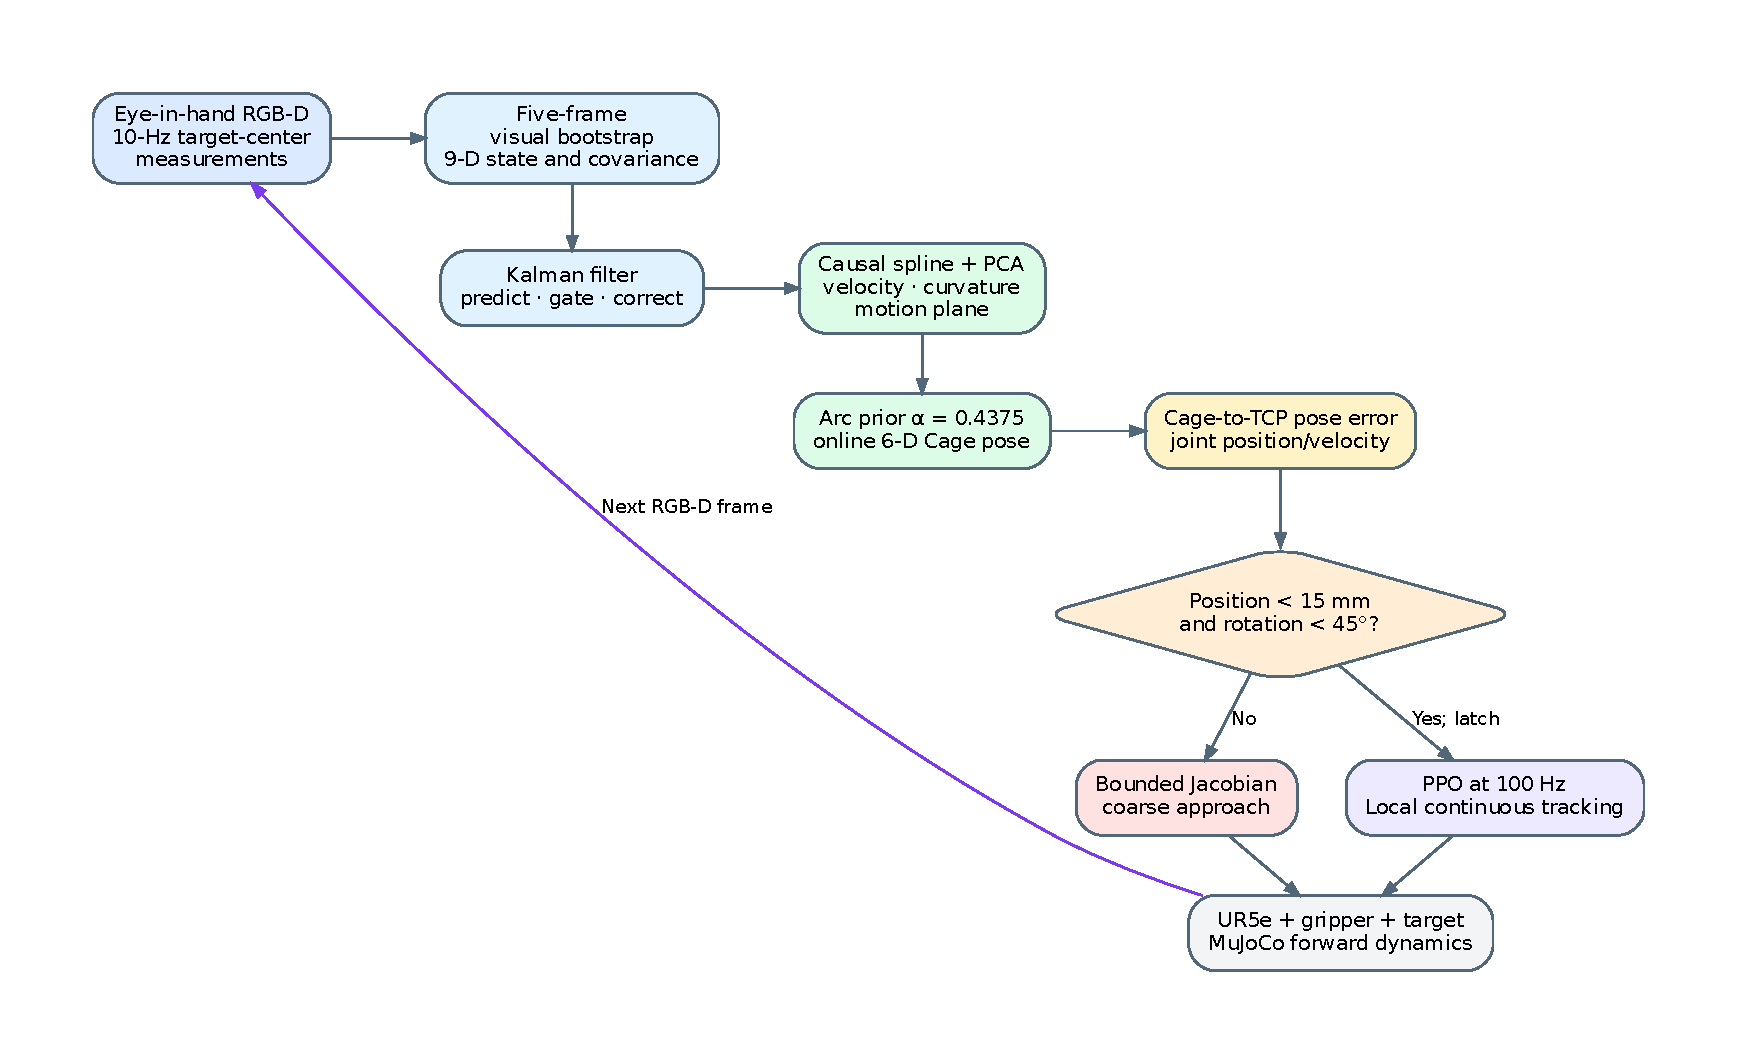
\includegraphics[width=0.96\textwidth]{system_pipeline_ieee.pdf}
\caption{System pipeline. Offline dynamics evaluation extracts a compact Cage-placement prior. Online RGB-D measurements are converted into a causal motion estimate and Cage pose at 10~Hz; the UR5e controller runs at 100~Hz and switches from Jacobian approach to latched PPO tracking.}
\label{fig:pipeline}
\end{figure*}

\section{Related Work}

\subsection{Moving-Target Visual Servoing}

Moving targets introduce an external feature velocity that causes steady tracking lag if it is ignored. Ito and Shibata reduced this delay through target-motion compensation on a three-degree-of-freedom planar eye-in-hand robot \cite{ito2009}. Shahriari \emph{et al.} adapted a depth observer to a moving target, estimating image-plane motion through a disturbance observer and the orthogonal component through focus of expansion \cite{shahriari2013}. Dong and Zhu combined eye-in-hand visual servoing with adaptive extended Kalman estimation for autonomous capture \cite{dong2016}. These methods motivate the explicit separation of measurement filtering, motion estimation, reference generation, and robot control adopted here.

\subsection{Caging and Dynamics-Based Evaluation}

Geometric caging limits object escape without requiring force closure. Dynamic-caging research has extended this idea to contact-rich motion using forward dynamics and robustness measures \cite{dong2024caging}. Our score is deliberately different: one Cage candidate is held fixed, target states are expanded under random disturbances, and the fraction of tree states inside the actual open U-shaped region is measured. The expansive-space-tree (EST) principle \cite{hsu1997} only favors low-density target states during this stress test; it does not plan a manipulator trajectory.

\subsection{Learned Joint-Space Control}

Inverse kinematics and Jacobian control are efficient and interpretable but require explicit treatment of singularities, joint limits, and velocity bounds. Learned joint-space control can represent nonlinear coupling directly. JAiLeR maps a task-space goal and joint state to joint commands using deep reinforcement learning \cite{kumar2021}. Our implementation follows that task-space-to-joint-space perspective while adding a finer curriculum, separate Actor and Critic optimizers, a stage-dependent exploration schedule, error-dependent action gain, and online Jacobian--PPO mode switching.

\section{Problem Formulation and Architecture}

\subsection{Frames and Objective}

All frames are right-handed. Let $\{B\}$, $\{T\}$, $\{K\}$, and $\{G\}$ denote the robot Base, TCP, camera, and physical gripper Cage frames. The camera and gripper are rigidly attached to the terminal link, so \({}^{T}\mathbf T_K\) and \({}^{T}\mathbf T_G\) are fixed calibrations. The desired dynamic Cage pose \({}^{B}\mathbf T^{*}_{C,k}\), in contrast, changes with the observed motion.

The RGB-D detector returns the center of a spherical target proxy. In homogeneous coordinates,
\begin{equation}
{}^{B}\bar{\mathbf p}_{o,k}
= {}^{B}\mathbf T_{K,k}\,{}^{K}\bar{\mathbf p}_{o,k},
\qquad
{}^{B}\mathbf T_{K,k}
= {}^{B}\mathbf T_{T,k}\,{}^{T}\mathbf T_K .
\label{eq:camera_to_base}
\end{equation}
The physical MuJoCo object has mass, radius, contact, and rigid-body dynamics; only its center is required for online Cage reconstruction. The desired TCP pose is obtained through the fixed gripper extrinsic:
\begin{equation}
{}^{B}\mathbf T^{*}_{T,k}
= {}^{B}\mathbf T^{*}_{C,k}
\left({}^{T}\mathbf T_G\right)^{-1}.
\label{eq:cage_to_tcp}
\end{equation}
The robot tracks this pose subject to joint, rate, collision, workspace, and visibility constraints.

\subsection{Multi-Rate State Machine}

The RGB-D clock is 10~Hz, joint commands are updated at 100~Hz, and MuJoCo integrates at 500~Hz. Target motion is independent of inference. During the first five valid images, the robot holds an observation pose and collects raw visual centers. Starting at frame six, the system reconstructs the Cage and uses a bounded Jacobian controller. PPO is latched when the position and shortest-rotation errors fall below 15~mm and $45^{\circ}$, respectively. One or two missing images invoke state prediction; three consecutive misses terminate the simulated task. Table~\ref{tab:system_contract} summarizes the execution contract.

\begin{table}[t]
\caption{Core System Contract}
\label{tab:system_contract}
\centering
\begin{tabular}{lr}
\toprule
Quantity & Value \\
\midrule
RGB-D update & 100 ms (10 Hz) \\
Joint-control update & 10 ms (100 Hz) \\
MuJoCo integration step & 2 ms \\
Estimator state & 9 dimensions \\
PPO state/action & 18 / 6 dimensions \\
PPO entry neighborhood & 15 mm, $45^{\circ}$ \\
Visual failure & 3 consecutive misses \\
\bottomrule
\end{tabular}
\end{table}

\section{Visual Motion and Cage Reconstruction}

\subsection{RGB-D Measurement and State Initialization}

The simulation camera renders $320\times240$ color and depth images. A red-color mask isolates the spherical object; valid foreground pixels are back-projected, and their median three-dimensional point is offset by the known 18-mm radius along the viewing direction. Center estimation is therefore an RGB-D measurement process, not direct access to the MuJoCo state.

The first valid image defines the beginning of an observation sequence, but a velocity is neither measured nor assumed at that instant. At the 10-Hz visual rate, the five centers \(P_1,\ldots,P_5\) span four sampling intervals, i.e., 0.4~s. For the configured 0.11--0.18~m/s motion range, this corresponds to approximately 44--72~mm of traveled arc length. The interval is therefore long enough to expose a measurable motion trend while remaining local relative to the complete trajectory. The nine-dimensional motion state is
\begin{equation}
\mathbf x_k =
\begin{bmatrix}
\mathbf p_k^{\mathsf T}&
\mathbf v_k^{\mathsf T}&
\mathbf a_k^{\mathsf T}
\end{bmatrix}^{\mathsf T}.
\label{eq:motion_state}
\end{equation}
The five valid centers are fitted jointly by a local quadratic model whose time origin is the newest measurement. The fit therefore initializes position, velocity, and acceleration at \(P_5\), rather than attempting to assign a reliable velocity to \(P_1\). During bootstrap, the first-frame provisional velocity may be zero and intermediate finite-difference velocities are diagnostic only; no Cage command depends on them. Fit residuals initialize the covariance, with standard-deviation floors of 3~mm, 0.03~m/s, and 0.20~m/s$^2$. This history-based initialization avoids imposing zero target velocity on the formal filter state.

From frame six, a constant-acceleration Kalman model with white-jerk process noise performs prediction and position correction \cite{kalman1960}. The innovation is accepted only when
\begin{equation}
d_k^2=\mathbf y_k^{\mathsf T}\mathbf S_k^{-1}\mathbf y_k
\leq 14.16.
\label{eq:innovation_gate}
\end{equation}
A missed or rejected measurement invokes prediction only and increases uncertainty; it does not erase the accumulated state. The configured observation variance is $9\times10^{-6}$~m$^2$.

\subsection{Causal Spline and Local Motion Plane}

A cubic B-spline is fitted over a finite causal window. The three coordinates share timestamps, knots, basis functions, and recency weights. The implemented fit is
\begin{equation}
\mathbf C^{*}=\arg\min_{\mathbf C}
\sum_i w_i
\left\|\mathbf b(t_i)^{\mathsf T}\mathbf C-\hat{\mathbf p}_i\right\|_2^2
+\lambda\left\|\mathbf D_2\mathbf C\right\|_F^2 ,
\label{eq:spline}
\end{equation}
where $\mathbf D_2$ penalizes second differences of the control coefficients. Kalman state variables provide online position, velocity, and acceleration; the spline supplies causal curve continuation, tangent fallback, and curvature
\begin{equation}
\kappa(t)=
\frac{\left\|\dot{\mathbf s}(t)\times\ddot{\mathbf s}(t)\right\|_2}
{\left\|\dot{\mathbf s}(t)\right\|_2^3}.
\label{eq:curvature}
\end{equation}

The centered covariance of recent curve samples has eigenvalues
$\lambda_1\leq\lambda_2\leq\lambda_3$. When $\lambda_2/\lambda_3$ indicates sufficient two-dimensional spread, the eigenvector of $\lambda_1$ defines the PCA plane normal \cite{jolliffe2002}. For sufficiently curved motion, the differential normal $\dot{\mathbf s}\times\ddot{\mathbf s}$ is also available. Near a line, the previous normal or a Base-frame reference is reused. Sign consistency and rotation bounds prevent eigenvector flips.

\subsection{Speed-Dependent Minor Arc}

The target center is the center of a candidate circle in the local motion plane. Its unfiltered speed-dependent radius is
\begin{equation}
\tilde r_k=0.10+
0.08\,\operatorname{clip}\!\left(
\frac{\|\mathbf v_k\|-0.05}{0.45-0.05},0,1
\right)\ \mathrm{m}.
\label{eq:speed_radius}
\end{equation}
At 10~Hz, $r_k=0.49r_{k-1}+0.51\tilde r_k$, followed by a physical rate limit of 0.18~m/s. The tangent--circle intersection defines the arc start; the first intersection of the causally continued curve and circle defines the end. For normalized coordinate $\alpha\in[0,1]$,
\begin{align}
\theta(\alpha)&=\theta_s+\alpha(\theta_e-\theta_s),\nonumber\\
\mathbf p_C(\alpha)&=\mathbf p_k+r_k
\left[\cos\theta(\alpha)\mathbf u_k+
\sin\theta(\alpha)\mathbf v_k\right].
\label{eq:arc}
\end{align}
The Cage $x$-axis points toward the object, its $z$-axis is the stabilized positive plane normal, and its $y$-axis completes a right-handed frame. Hence the Cage $x$--$y$ plane is parallel to the local motion plane.

\section{Offline Dynamics-Based Cage Experience}

\subsection{Candidates and EST Expansion}

For offline experience generation, the first five trajectory points are retained as causal geometric history but do not produce Cage labels. The first valid label is generated at \(P_6\). Because \(P_1\) to \(P_6\) spans five 0.1-s intervals, the clean object has traveled approximately 55--90~mm before the first label under the configured speed range. Velocity, acceleration, tangent, and curvature at \(P_6\) are obtained from the smooth trajectory fit rather than from a separately specified first-frame velocity. Nine candidates then uniformly sample the exact minor arc. The clean generated trajectory supplies the privileged future segment needed to locate the arc endpoint; this is confined to offline label construction. Online reconstruction uses only causal spline continuation.

One candidate remains fixed during each EST trial. The root contains current object position and linear velocity. EST selects parents preferentially from sparsely occupied cells of a position--linear-velocity--angular-velocity grid. A random force, torque, and duration are applied, and MuJoCo performs forward integration. Seventy percent of force directions point into the current motion-arc sector, while 30\% preserve global three-dimensional exploration. Each candidate receives the same three disturbance tapes, 640 nodes per repeat, a 0.8-s horizon, and a 5-ms integration step.

Valid states are classified against the actual rear wall, open mouth, width, and height of the U-shaped gripper. Nonfinite states, local-bound violations, and penetration beyond 6~mm are not expanded. The full procedure is shown in Fig.~\ref{fig:est}.

\begin{figure*}[t]
\centering
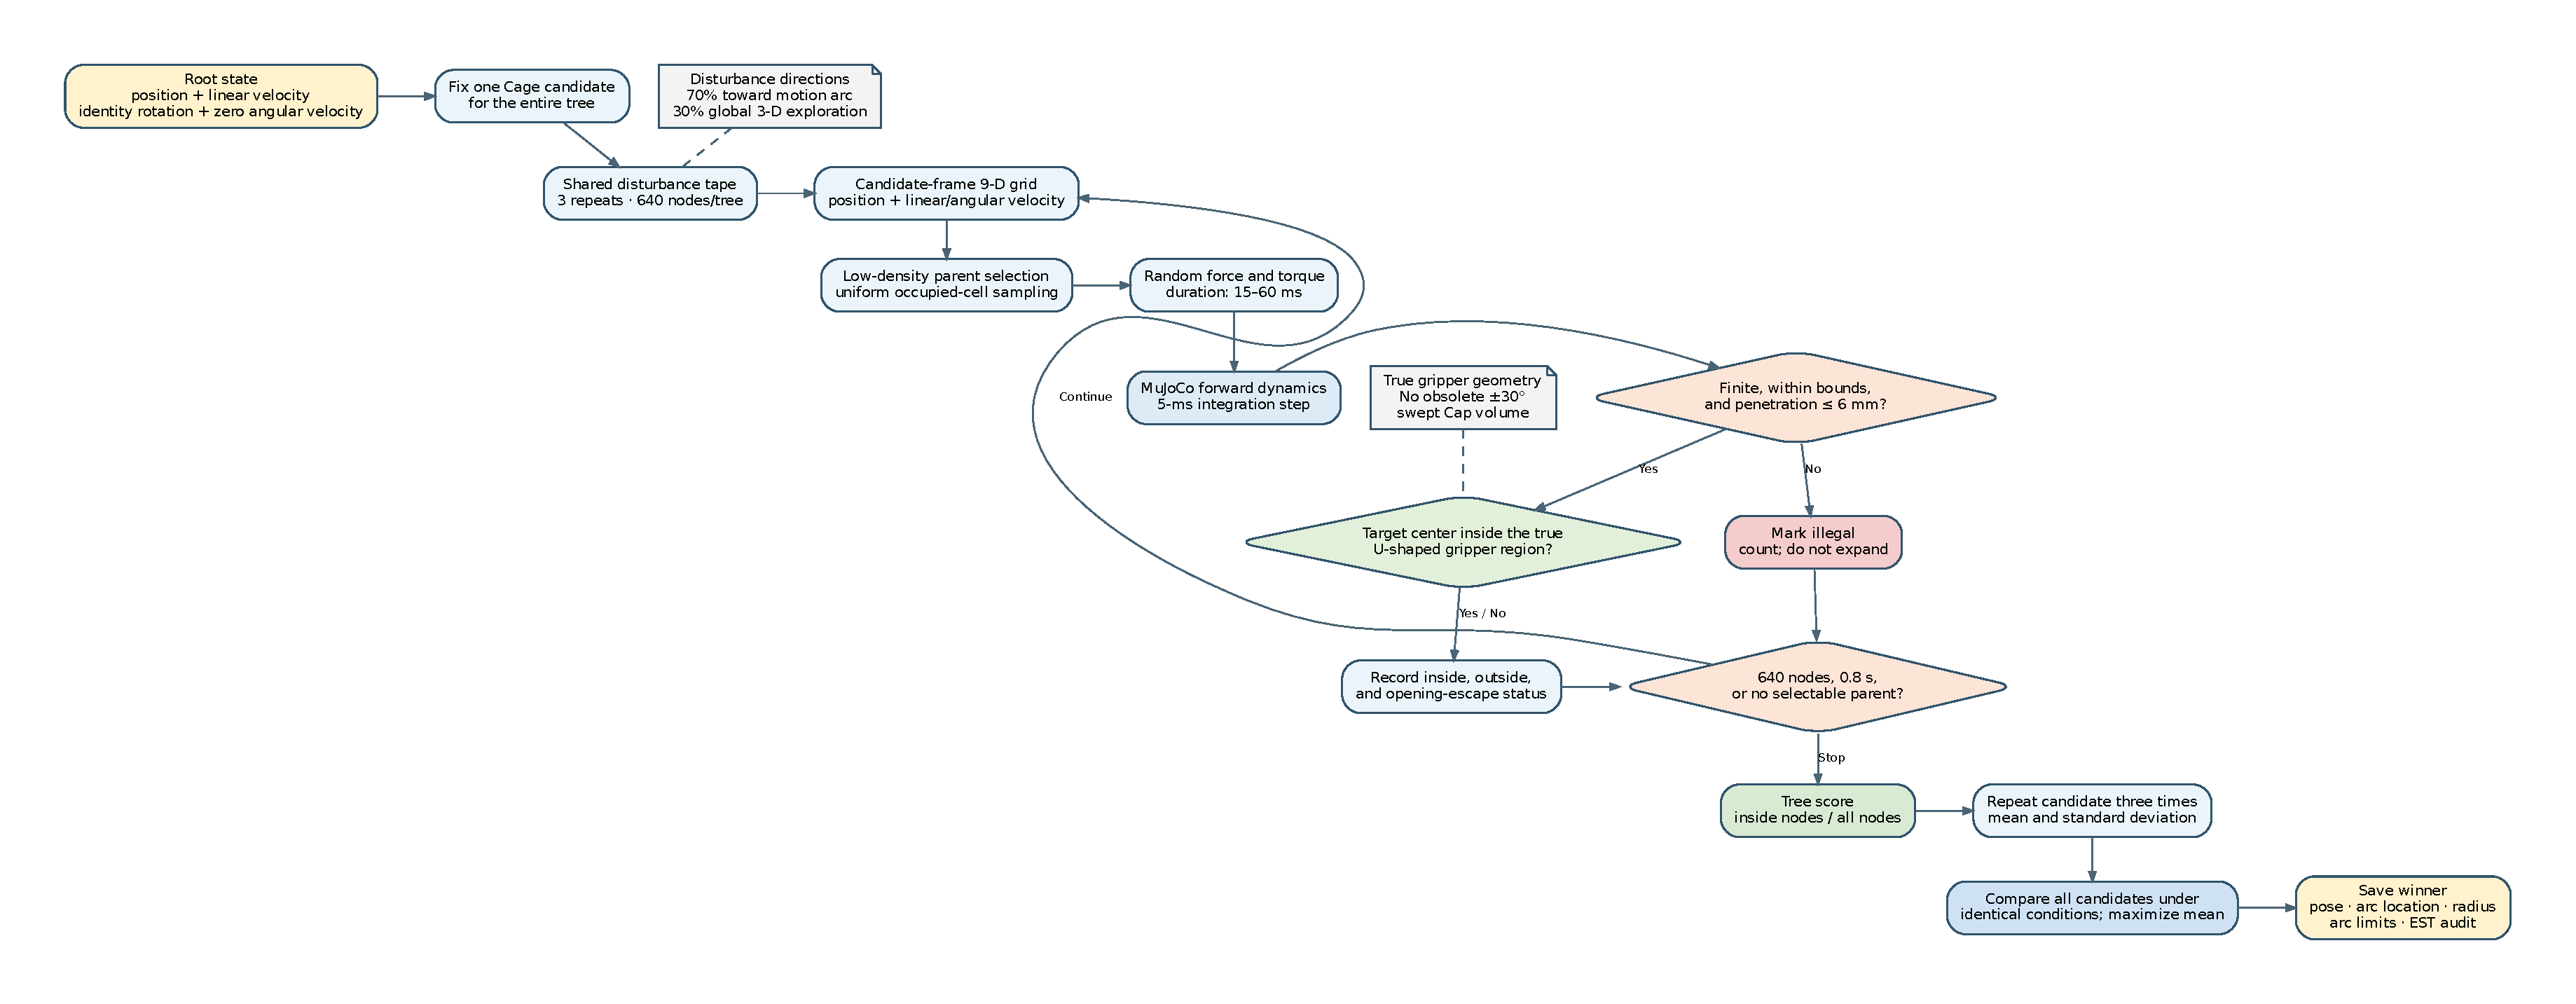
\includegraphics[width=0.95\textwidth]{est_expansion_flow_ieee.pdf}
\caption{Offline evaluation of one fixed Cage candidate. EST expands object dynamics only. Candidate pose, gripper geometry, node budget, and disturbance tape remain controlled so that candidates are directly comparable.}
\label{fig:est}
\end{figure*}

For candidate $j$ and repeat $m$,
\begin{equation}
\rho_{j,m}=\frac{N^{\mathrm{in}}_{j,m}}{N_{j,m}},
\quad
\bar\rho_j=\frac{1}{3}\sum_{m=1}^{3}\rho_{j,m},
\quad
\sigma_j=\operatorname{Std}(\rho_{j,1:3}).
\label{eq:est_score}
\end{equation}
The final label is
\begin{equation}
j^{*}=\arg\max_{j\in\mathcal F}\bar\rho_j ,
\label{eq:est_selection}
\end{equation}
where $\mathcal F$ is the feasible set and the winner must exceed the nonzero-retention threshold. IK margin, joint change, temporal continuity, pose smoothness, and arc midpoint are not secondary ranking terms; the candidate index only resolves an exact tie.

\subsection{Compact Online Prior}

The archive contains 55,121 valid labels from 2,919 trajectories. The winning $\alpha$ has mean 0.402 and median 0.375. An all-candidate audit of 10,000 labels shows that fixed $\alpha=0.5$ has the largest mean occupancy. Absolute correlations of the winner with speed, acceleration, curvature, and radius are below 0.02. Figure~\ref{fig:arc_prior} therefore supports a fixed prior more strongly than a state-conditioned regressor for the present gripper and disturbance distribution. The online reconstruction uses $\alpha=0.4375$, halfway between the empirical median and the best fixed audit candidate.

\begin{figure*}[t]
\centering
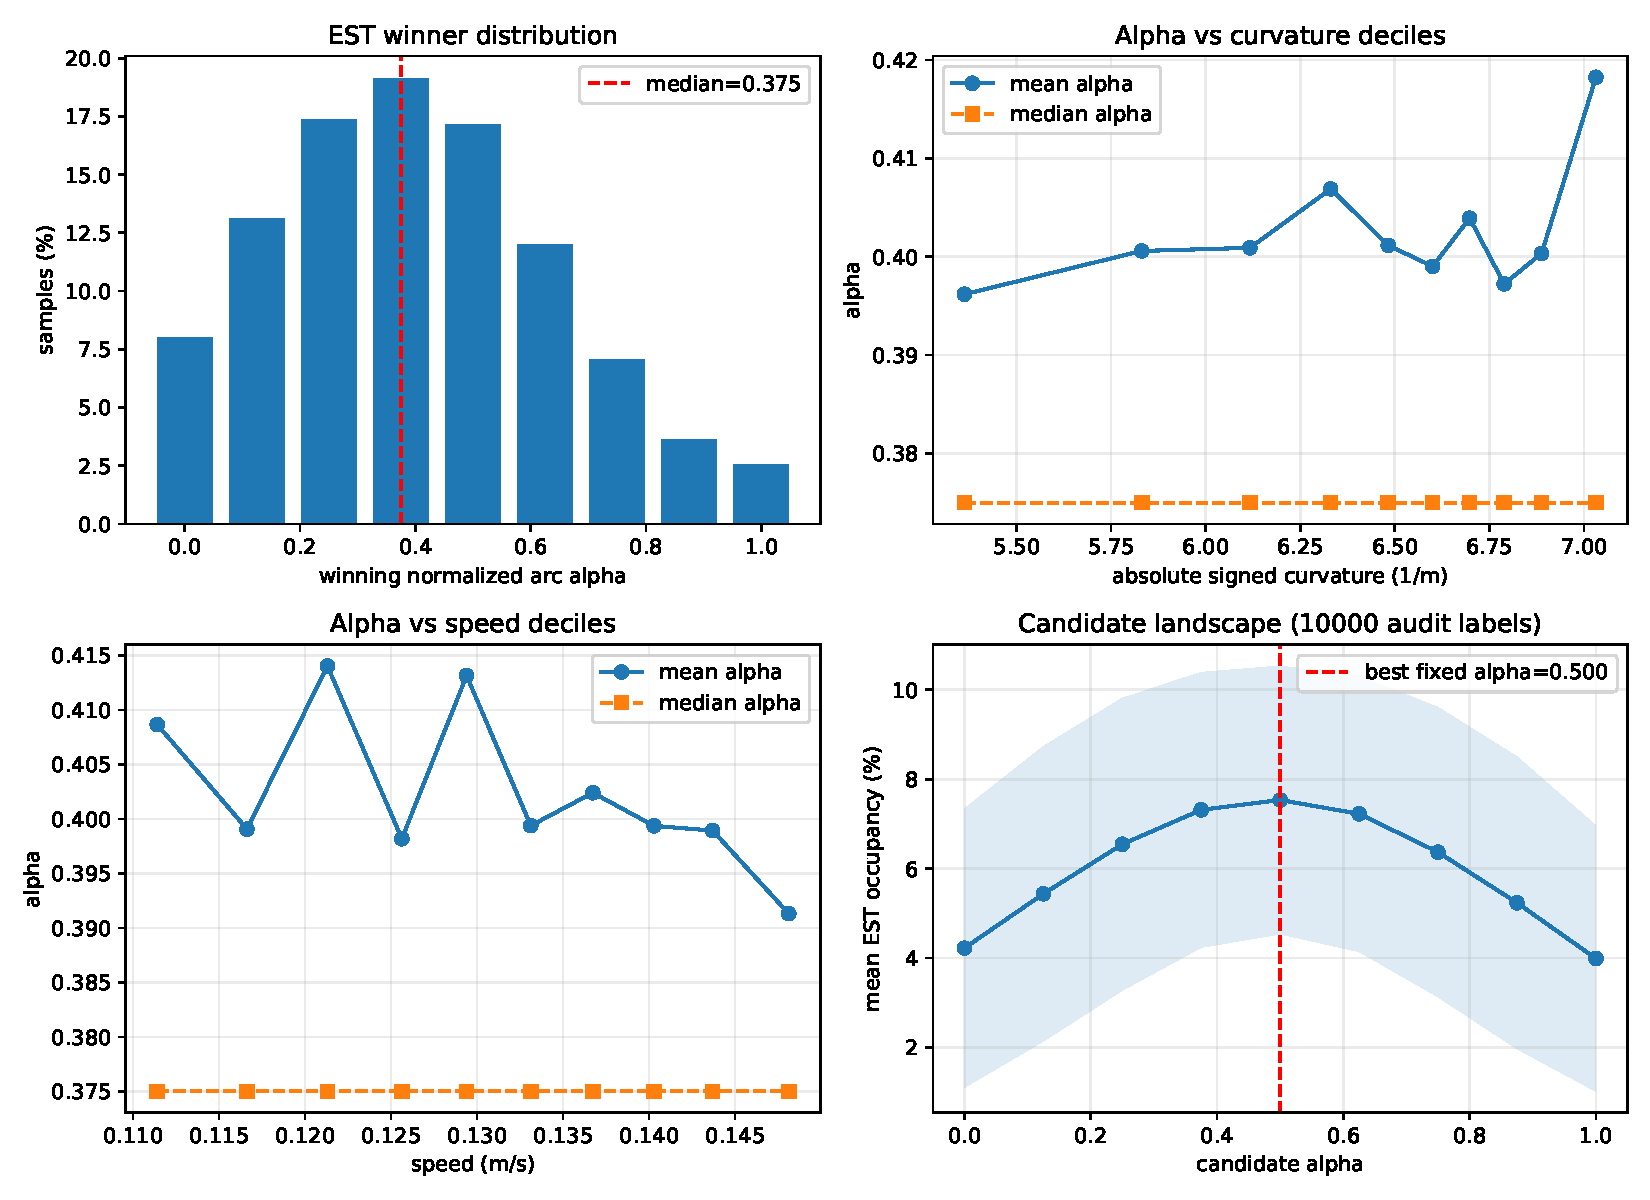
\includegraphics[width=0.96\textwidth]{state_arc_prior_relationships_ieee.pdf}
\caption{Offline state--arc audit. Winners are centered near the middle of the minor arc, while their measured dependence on the tested motion variables is weak.}
\label{fig:arc_prior}
\end{figure*}

\section{Hybrid Control and Policy Training}

\subsection{Bounded Jacobian Approach}

Let $\mathbf e_p$ be the Base-frame TCP position error and $\mathbf e_R$ the shortest rotation-vector error. The desired Cartesian twist is
\begin{equation}
\boldsymbol\xi^{*}=\boldsymbol\xi_{\mathrm{ff}}+
\begin{bmatrix}k_p\mathbf e_p&k_R\mathbf e_R\end{bmatrix}^{\mathsf T}.
\label{eq:twist}
\end{equation}
The approach controller solves a bounded damped least-squares problem \cite{wampler1986}:
\begin{equation}
\dot{\mathbf q}^{*}=
\arg\min_{\dot{\mathbf q}}
\|\mathbf W(\mathbf J\dot{\mathbf q}-\boldsymbol\xi^{*})\|_2^2
+\lambda_J\|\dot{\mathbf q}\|_2^2 ,
\quad
\dot{\mathbf q}_{\min}\leq\dot{\mathbf q}\leq\dot{\mathbf q}_{\max}.
\label{eq:jacobian}
\end{equation}
The bounds include speed, acceleration, and remaining joint-position margins. This phase provides predictable large-error convergence without requiring PPO to discover long-range inverse kinematics.

\subsection{PPO State, Network, and Action}

The policy state is
\begin{equation}
\mathbf s_t=
\begin{bmatrix}
\mathbf e_{p,t}^{\mathsf T}&
\mathbf e_{R,t}^{\mathsf T}&
\mathbf q_t^{\mathsf T}&
\dot{\mathbf q}_t^{\mathsf T}
\end{bmatrix}^{\mathsf T}\in\mathbb R^{18}.
\label{eq:ppo_state}
\end{equation}
Running means and variances normalize the state. Actor and Critic have independent $18\!\rightarrow\!128\!\rightarrow\!128$ multilayer perceptrons with $\tanh$ hidden activations. The Actor outputs six means and maintains six trainable state-independent log standard deviations; the Critic outputs one state value. Figure~\ref{fig:ppo} shows both paths.

\begin{figure*}[t]
\centering
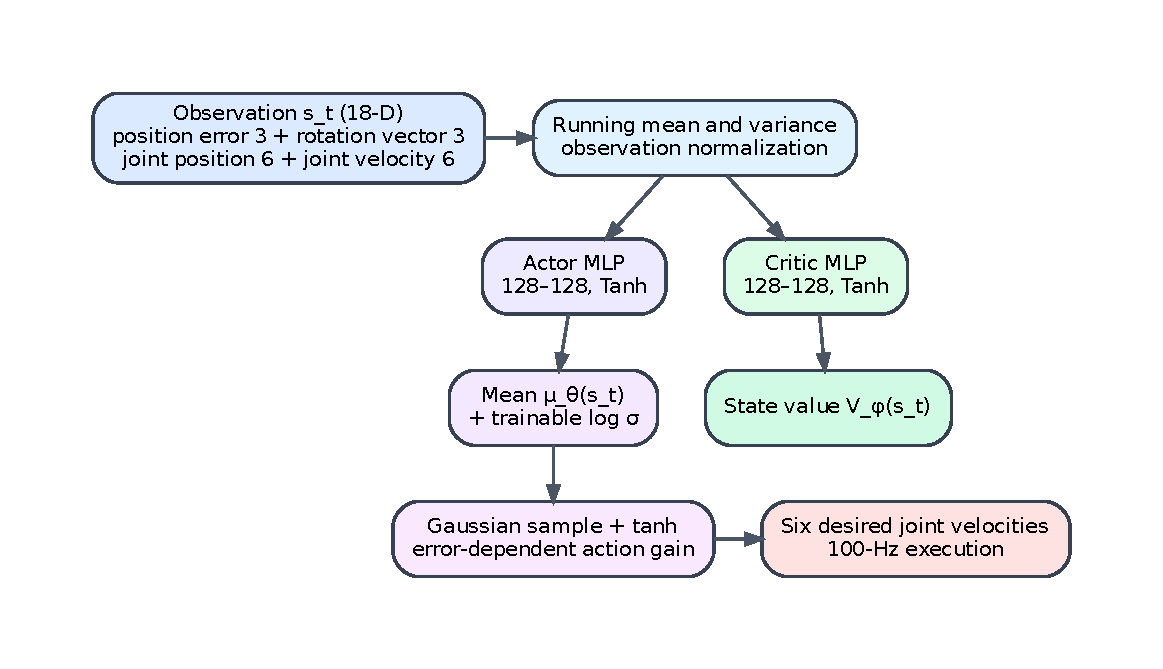
\includegraphics[width=0.90\textwidth]{ppo_architecture_ieee.pdf}
\caption{Independent Actor and Critic paths. The Actor produces a bounded normalized six-joint action, and the state-dependent gain converts it into a 100-Hz physical joint-velocity command.}
\label{fig:ppo}
\end{figure*}

The latent and squashed actions are
\begin{equation}
\mathbf u_t\sim\mathcal N(\boldsymbol\mu_\theta(\bar{\mathbf s}_t),
\operatorname{diag}(\boldsymbol\sigma_\theta^2)),
\qquad
\mathbf a_t=\tanh(\mathbf u_t).
\label{eq:action}
\end{equation}
The actual squashed-action density includes the change-of-variables correction:
\begin{equation}
\log\pi_\theta(\mathbf a_t|\mathbf s_t)=
\log\mathcal N(\operatorname{atanh}\mathbf a_t;
\boldsymbol\mu_\theta,\boldsymbol\sigma_\theta)
-\sum_i\log(1-a_{t,i}^2+\varepsilon).
\label{eq:density}
\end{equation}

The policy output is a normalized joint velocity, not a one-step target displacement. At every 10-ms control step,
\begin{align}
d_t&=\max\!\left(
\frac{\|\mathbf e_{p,t}\|}{\delta_p},
\frac{\|\mathbf e_{R,t}\|_{\mathrm{deg}}}{\delta_R}\right),\nonumber\\
g_t&=\min\{g_{\mathrm{stage}},\mathcal I(d_t)\},\nonumber\\
\dot{\mathbf q}_{\mathrm{cmd},t}
&=\dot{\mathbf q}_{\mathrm{lim}}\odot(g_t\mathbf a_t).
\label{eq:gain}
\end{align}
For position stages the orientation ratio is omitted. $\mathcal I$ linearly interpolates
\[
(d,g)=\{(0,0.10),(0.5,0.10),(1,0.20),(2,0.40),(4,0.70),(6,1.00)\}.
\]
Thus the more severe normalized pose error controls one common physical speed gain: commands are gentle near the goal and faster at larger error.

\subsection{PPO, Critic, and Exploration Entropy}

After every rollout, temporal-difference residuals, generalized advantages \cite{schulman2015gae}, and Critic targets are computed once from frozen old values:
\begin{align}
\delta_t&=r_t+\gamma(1-b_t)V_{\mathrm{old}}(s_{t+1})
-V_{\mathrm{old}}(s_t),\nonumber\\
\hat A_t&=\sum_{l\geq0}(\gamma\lambda)^l\delta_{t+l},
\qquad
\hat V_t=V_{\mathrm{old}}(s_t)+\hat A_t .
\label{eq:gae}
\end{align}
Here $b_t$ marks a true physical terminal; a time limit retains value bootstrap. Both labels remain fixed through all minibatch epochs of one update.

With probability ratio $r_t(\theta)$, the Actor maximizes
\begin{equation}
J_\pi(\theta)=\mathbb E_t\!\left[
\min\!\left(r_t\hat A_t^n,
\operatorname{clip}(r_t,1-\epsilon,1+\epsilon)\hat A_t^n\right)
+\beta\mathcal H(\pi_\theta)
\right],
\label{eq:ppo}
\end{equation}
where $\hat A_t^n$ is normalized and
$\mathcal H=-\mathbb E_{\pi_\theta}[\log\pi_\theta]$ is evaluated for the squashed policy. The Critic independently minimizes
\begin{equation}
L_V(\phi)=\frac{1}{2}\mathbb E_t
\left[(V_\phi(s_t)-\hat V_t)^2\right].
\label{eq:critic}
\end{equation}
Separate Adam optimizers use learning rates $2\times10^{-5}$ and $10^{-4}$. Each update permits eight Actor epochs and twelve Critic epochs with 512-sample minibatches. PPO uses $\epsilon=0.2$. Approximate KL above 0.03 stops only Actor epochs; Critic regression continues. Clipping is therefore a local sample-wise restriction, while KL stopping limits the aggregate policy change.
\begin{equation}
\widehat D_{\mathrm{KL}}
=\mathbb E_t\!\left[(r_t-1)-\log r_t\right].
\label{eq:approx_kl}
\end{equation}

Within stage $s$, the entropy coefficient follows
\begin{equation}
\beta_s(n)=m_s(n)\!\left[
\beta_s^{0}+
\min\!\left(\frac{n}{N_s},1\right)
(\beta_s^{1}-\beta_s^{0})
\right],
\qquad \beta_s^{1}=\frac{1}{2}\beta_s^{0}.
\label{eq:entropy}
\end{equation}
Start values increase with task range: 0.0008--0.0018 in position passes and 0.0010--0.0030 in pose stages. The schedule encourages diverse actions early in a stage and precision later. After 20 updates with less than 2\% improvement, a pre-update Critic explained variance of at least 0.30 permits a 20-update entropy pulse $m_s=1.5$, at most three times per stage. A regression larger than 1\% never triggers more exploration. The trainable log standard deviations are optimized by \eqref{eq:ppo}; the plateau detector does not permanently overwrite them.

\subsection{Overall Reward}

For $e_p=\|\mathbf e_p\|$, position quality combines a millimeter-sensitive term and a long-tail term:
\begin{align}
Q_{p,f}&=\exp\!\left[-\ln2(e_p/\delta_p)^2\right],\nonumber\\
Q_{p,c}&=\frac{1}{1+(e_p/e_{p,\max})^2},\nonumber\\
Q_p&=0.7Q_{p,f}+0.3Q_{p,c}.
\label{eq:position_quality}
\end{align}
The fine term equals 0.5 at the current success threshold and separates nearby millimeter errors. The inverse-quadratic term avoids the nearly zero, indistinguishable quality that one narrow exponential would assign to all distant states.

Orientation uses three 5-cm virtual markers anchored at one common origin:
\begin{equation}
E_R=\frac{1}{3}\sum_{i=1}^{3}
\|\ell\mathbf R\mathbf e_i-\ell\mathbf R^*\mathbf e_i\|_2^2,
\qquad
Q_R=\frac{1}{1+40000E_R},
\quad \ell=0.05\ \mathrm m.
\label{eq:orientation_quality}
\end{equation}
The common origin prevents translation from being counted twice, and the inverse-quadratic quality retains variation after large wrist errors.

In pose stages, let $u_p=e_p/\delta_p$ and
$u_R=e_R^{\mathrm{deg}}/\delta_R$. Before either component succeeds,
\begin{equation}
w_R=\operatorname{clip}
\left(\frac{u_R}{u_p+u_R},0.25,0.75\right),
\qquad w_p=1-w_R.
\label{eq:weights}
\end{equation}
If exactly one component succeeds, it retains weight 0.25 and the unfinished component receives 0.75; both receive 0.5 after joint success. Position stages use $(w_p,w_R)=(1,0)$.

Progress is the signed reduction over consecutive states:
\begin{align}
P_p&=\operatorname{clip}
\left(\frac{e_{p,t-1}-e_{p,t}}{0.005},-1,1\right),\nonumber\\
P_R&=\operatorname{clip}
\left(\frac{e_{R,t-1}-e_{R,t}}{10^{\circ}},-1,1\right).
\label{eq:progress}
\end{align}
Once one component is successful, its positive progress is removed but regression remains negative. The complete reward is
\begin{equation}
r_t=0.1(w_pQ_p+w_RQ_R-1)
+2w_pP_p+4w_RP_R-0.001C_a+R_{\mathrm{term}},
\label{eq:reward}
\end{equation}
where $C_a$ is normalized desired joint-acceleration cost. Success adds $+10$. Collision, workspace violation, or a nonfinite state adds $-10$ and the discounted remaining baseline cost, preventing early failure from avoiding future step costs.

\subsection{Curriculum}

Fifty logical slots maintain independent UR5e states. Each slot receives one randomized complete task per rollout, so a quickly solved task cannot be repeatedly counted. Table~\ref{tab:curriculum} summarizes 30 stages. The masked pass learns position control with rotation inputs set to zero. The observed pass exposes rotation inputs while retaining a position objective. At phase changes, Actor weights are retained, Adam history is cleared, and a new Critic is aligned to the new rollout distribution. The joint pass then learns coupled position and orientation correction.

\begin{table*}[t]
\caption{Curriculum Ranges and Promotion Contract}
\label{tab:curriculum}
\centering
\footnotesize
\setlength{\tabcolsep}{3pt}
\begin{tabular}{@{}lccclp{5.3cm}@{}}
\toprule
Pass & Stages & Initial position & Initial rotation & Horizon & Success and promotion contract \\
\midrule
Masked position & M01--M10 & 6--20 to 6--150 mm & masked & 80--200 & Per-task position: 1.5--4.0 mm. Promote when last-10 success is at least 75\% and mean position is 2.3--8.0 mm. \\
Observed position & V01--V10 & 6--20 to 6--150 mm & observed & 80--200 & Same position-only contract; rotation enters the observation but not the success test. \\
Joint pose & J01--J10 & 6--20 to 6--150 mm & 0.5--5 to 0.5--45$^{\circ}$ & 100--250 & Per-task: 1.5--4.0 mm and 2.8--4.5$^{\circ}$. Promote at 75\% with means 2.3--8.0 mm and 3.4--6.5$^{\circ}$. \\
\bottomrule
\end{tabular}
\end{table*}

\section{Experiments}

\subsection{Simulation and Perception Errors}

Experiments use the MuJoCo UR5e model \cite{todorov2012}, \texttt{attachment\_site} as TCP, a rigid U-shaped gripper, and an eye-in-hand camera. Dynamic trajectories last 5--7~s, have speed 0.11--0.18~m/s with 10\%--20\% smooth modulation, and are filtered for workspace and visibility. Their generated coordinates are hidden from online estimation.

The rendered measurements contain 2-mm depth noise, 1\% pixel-depth dropout, finite-resolution quantization, and 1\% whole-frame dropout. These errors change both position measurements and derived motion quantities, so Kalman filtering is not a cosmetic post-process: it estimates unobserved velocity and acceleration, propagates through short misses, and weights inconsistent centers through \eqref{eq:innovation_gate}. This paper does not claim a numerical advantage over a no-filter baseline, because that ablation remains to be conducted.

Three evidence levels are kept separate. The EST archive supports the arc prior. Curriculum rollouts evaluate randomized Cage-reaching tasks and are not reported as dynamic-tracking generalization. The online sequence demonstrates executable integration of noisy RGB-D, causal Cage reconstruction, and controller switching.

\subsection{Curriculum Results}

The completed run contains 34,745 updates and passes all 30 stages. Figure~\ref{fig:curriculum} reports equally weighted last-ten-update statistics and promotion boundaries. The best final-stage checkpoint occurs at update 34,547. Table~\ref{tab:best} reports its completed-task result: 92\% success, 2.95-mm mean terminal position error, 3.94$^{\circ}$ mean terminal rotation error, 1.97\% action saturation, and 0.997 post-update Critic explained variance.

\begin{figure*}[t]
\centering
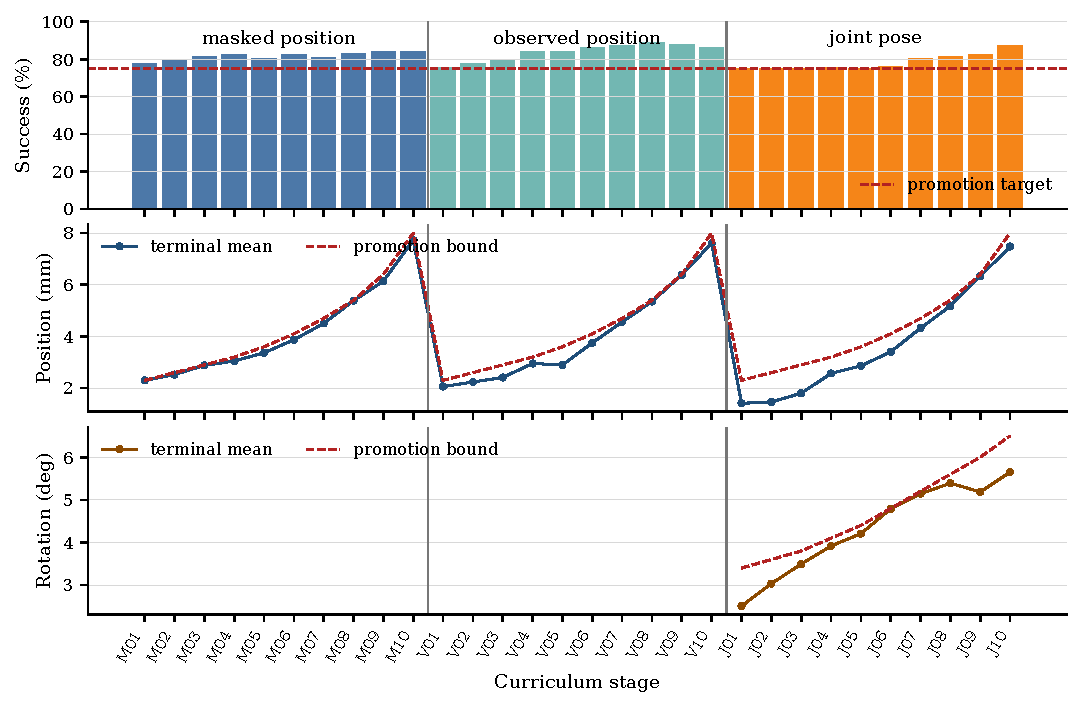
\includegraphics[width=0.96\textwidth]{curriculum_summary_ieee.pdf}
\caption{Per-stage last-ten-update statistics. Vertical dividers separate masked-position, observed-position, and joint-pose passes. Every completed task has equal weight.}
\label{fig:curriculum}
\end{figure*}

\begin{table}[t]
\caption{Best Final-Stage Checkpoint}
\label{tab:best}
\centering
\begin{tabular}{lr}
\toprule
Metric & Result \\
\midrule
Completed-task success & 92\% \\
Position mean / P95 & 2.95 / 4.00 mm \\
Rotation mean / P95 & 3.94 / 4.83$^{\circ}$ \\
Action saturation & 1.97\% \\
Critic explained variance & 0.997 \\
\bottomrule
\end{tabular}
\end{table}

\subsection{Online Tracking Sequence}

Figure~\ref{fig:inference} shows the causal execution phases. During bootstrap, the arm holds while raw RGB-D centers accumulate. At frame six, the initialized state and local curve produce the first Cage and the Jacobian controller performs coarse approach. After the entry thresholds are met, PPO is latched and supplies 100-Hz local joint-velocity corrections. The object and camera continue updating in every phase, and neither controller accesses generated future trajectory points.

\begin{figure*}[t]
\centering
\subfloat[Five-frame visual bootstrap; the arm holds.]{
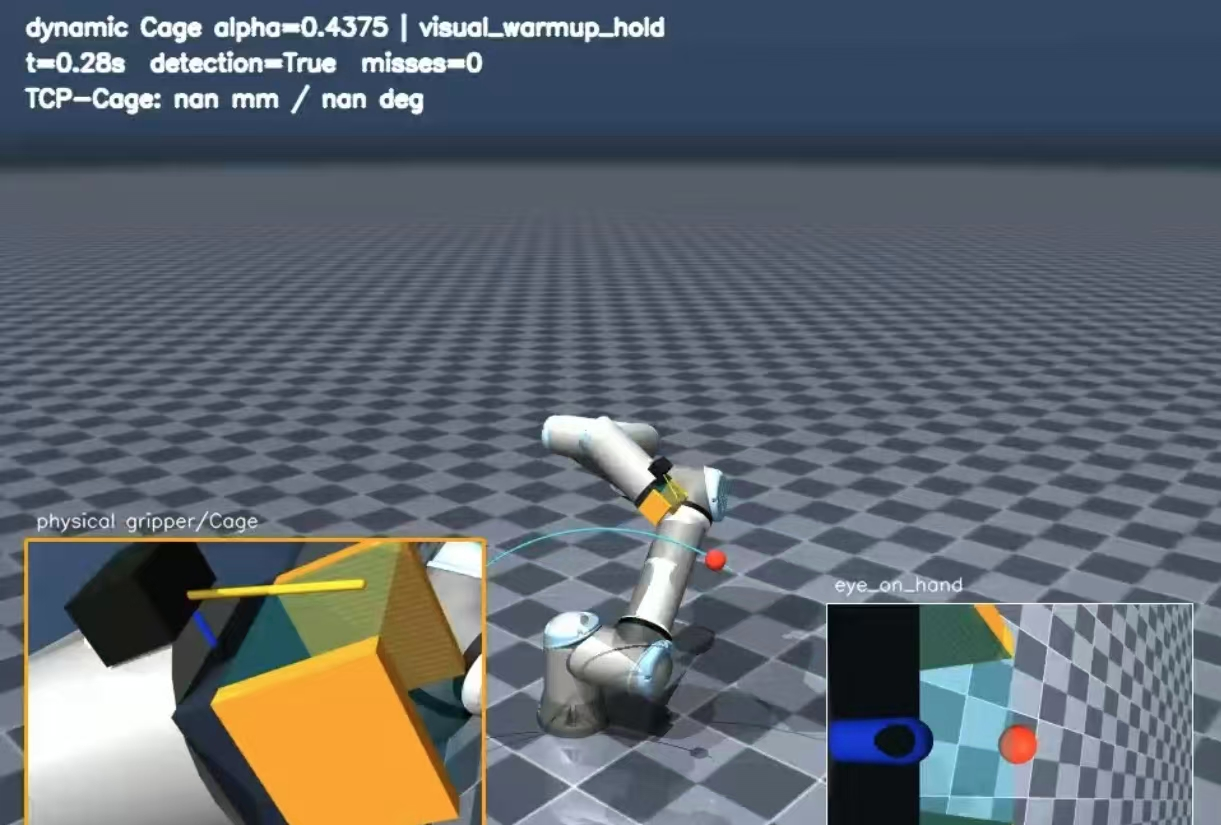
\includegraphics[width=0.47\textwidth]{inference_warmup.jpg}
\label{fig:warmup}}
\hfill
\subfloat[Cage reconstruction and Jacobian approach.]{
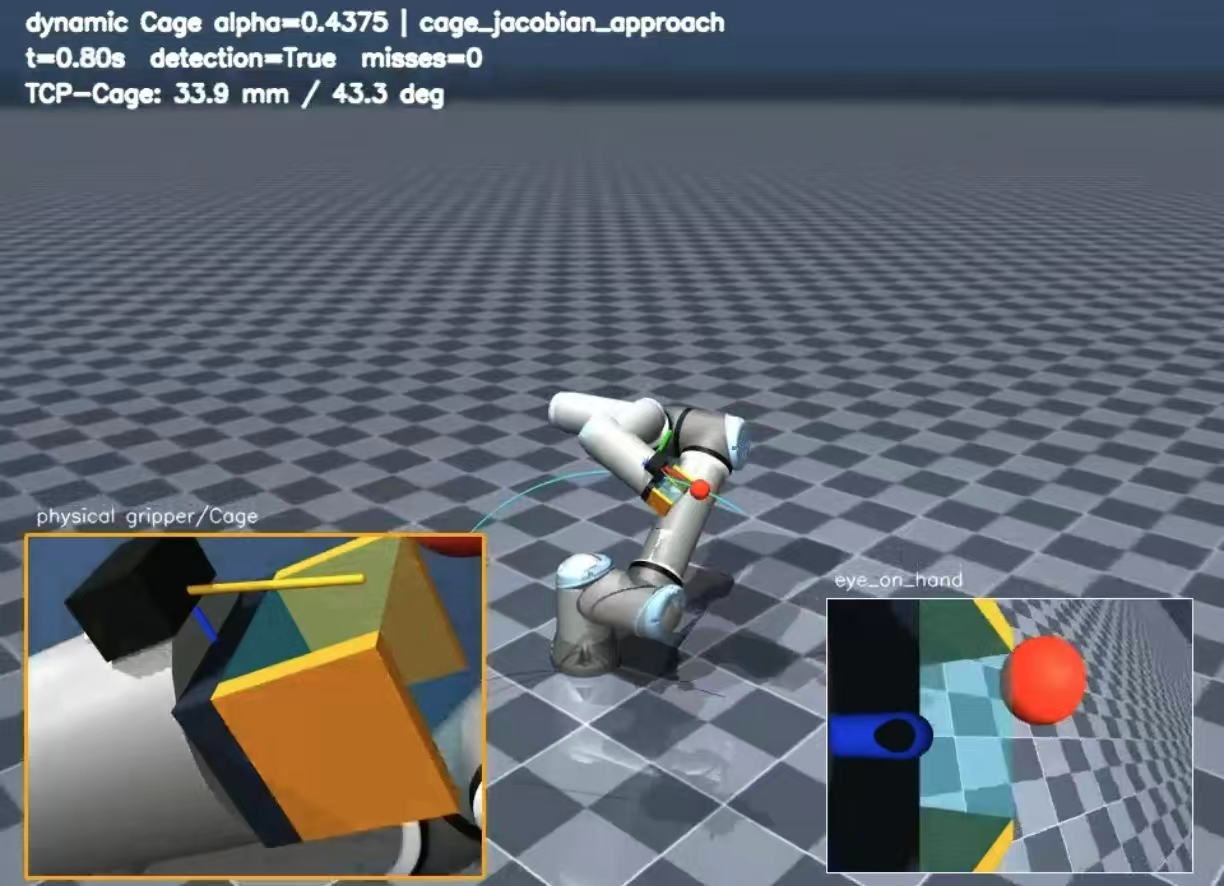
\includegraphics[width=0.47\textwidth]{inference_jacobian.jpg}
\label{fig:jacobian_frame}}\\[1mm]
\subfloat[Latched PPO local tracking.]{
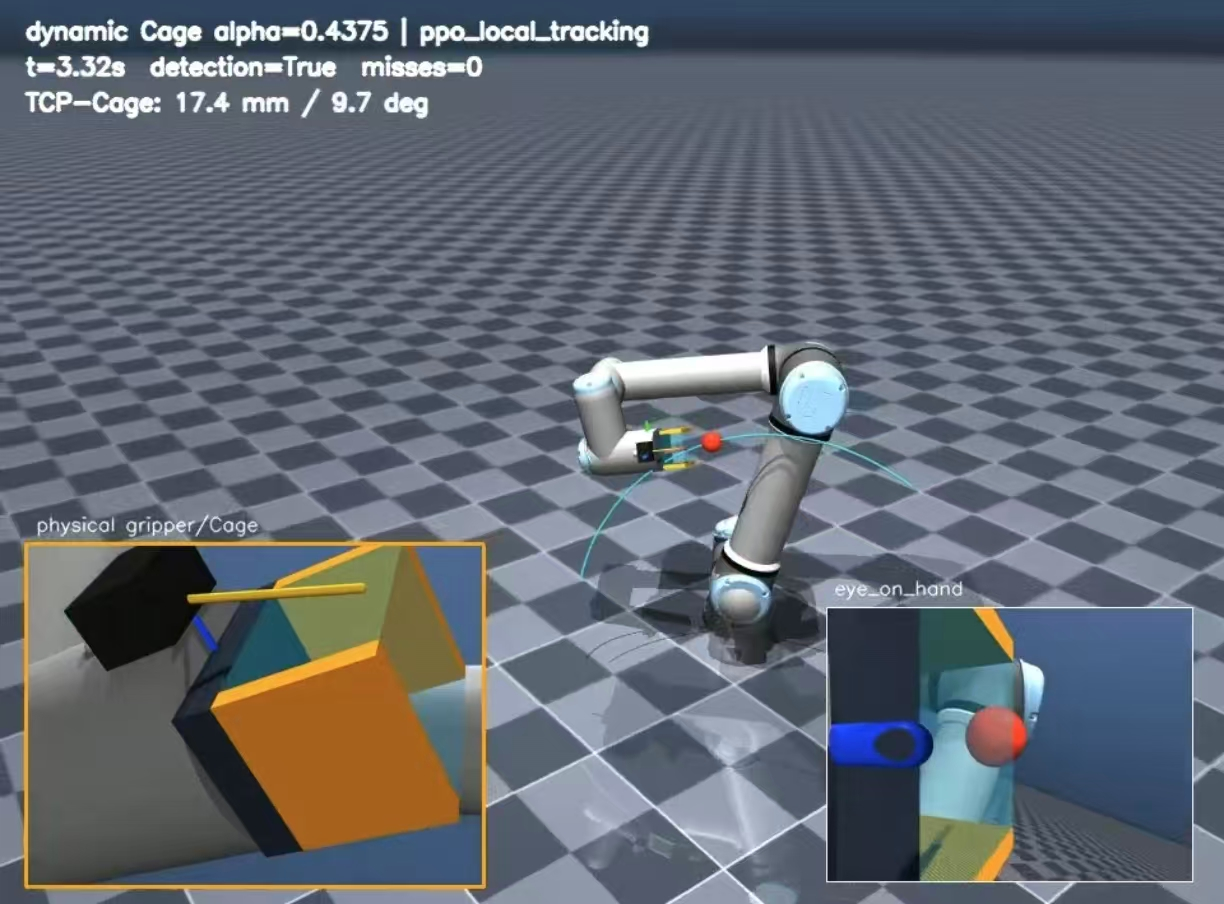
\includegraphics[width=0.47\textwidth]{inference_ppo.jpg}
\label{fig:ppo_frame}}
\caption{Representative MuJoCo inference sequence. Original frames are placed directly at readable size instead of being embedded in a small composite graphic.}
\label{fig:inference}
\end{figure*}

\section{Discussion}

The design separates expensive robustness experience from online computation. EST evaluates the interaction of disturbances and real gripper geometry offline. The weak measured state--winner relation supports a fixed prior for the current physical setting. Online computation is then limited to RGB-D center extraction, nine-dimensional filtering, local curve and plane estimation, one pose reconstruction, and robot control.

The controller similarly separates responsibilities. Jacobian control retains deterministic, constraint-aware large-error motion. PPO is used where nonlinear learned correction and repeated fast inference are most useful: inside a local moving-reference neighborhood. Error-dependent gain prevents one normalized action from producing excessive motion near the goal.

Limitations remain. Color segmentation is a controlled substitute for a real detector. Calibration drift, class ambiguity, and realistic occlusion are not yet represented. The fixed arc prior is specific to the present object, gripper, disturbance distribution, and speed range. Dynamic tracking currently has qualitative sequence evidence rather than a statistically powered benchmark. Future work will therefore add fixed-seed Jacobian-only, PPO-only, no-filter, and alternative-prior comparisons, followed by ROS-controlled physical UR5e experiments.

\section{Conclusion}

This paper presented a motion-aware dynamic Cage framework for continuous moving-object tracking. Offline rigid-body simulation evaluates Cage placements under identical disturbances and actual open-gripper geometry. Online RGB-D observations initialize and update a causal motion estimate from which a six-dimensional Cage is reconstructed. A bounded Jacobian controller handles large errors, and a curriculum-trained PPO policy supplies dynamically scaled local joint-velocity correction. The formulation makes the coordinate transforms, visual uncertainty, selection rule, policy density, exploration entropy, reward allocation, and evidence boundaries explicit. The resulting architecture combines stable long-range approach with agile local tracking without repeating the expensive dynamics search online.

\begin{thebibliography}{00}
\bibitem{ito2009}
M. Ito and M. Shibata, \lq\lq Image-based visual tracking control of hand-eye robot for moving target object,\rq\rq\ \emph{IEEJ Trans. Ind. Appl.}, vol. 129, no. 9, pp. 930--937, 2009, doi: 10.1541/ieejias.129.930.
\bibitem{shahriari2013}
N. Shahriari, S. Fantasia, F. Flacco, and G. Oriolo, \lq\lq Robotic visual servoing of moving targets,\rq\rq\ in \emph{Proc. IEEE/RSJ Int. Conf. Intell. Robots Syst. (IROS)}, 2013, pp. 77--82, doi: 10.1109/IROS.2013.6696335.
\bibitem{dong2016}
G. Dong and Z. H. Zhu, \lq\lq Autonomous robotic capture of non-cooperative target by adaptive extended Kalman filter based visual servo,\rq\rq\ \emph{Acta Astronaut.}, vol. 122, pp. 209--218, 2016, doi: 10.1016/j.actaastro.2016.02.003.
\bibitem{kumar2021}
V. Kumar, D. Hoeller, B. Sundaralingam, J. Tremblay, and S. Birchfield, \lq\lq Joint space control via deep reinforcement learning,\rq\rq\ in \emph{Proc. IEEE/RSJ Int. Conf. Intell. Robots Syst. (IROS)}, 2021, pp. 3619--3626.
\bibitem{schulman2017ppo}
J. Schulman, F. Wolski, P. Dhariwal, A. Radford, and O. Klimov, \lq\lq Proximal policy optimization algorithms,\rq\rq\ arXiv:1707.06347, 2017.
\bibitem{dong2024caging}
Y. Dong, X. Cheng, and F. T. Pokorny, \lq\lq Caging in motion: Characterizing robustness in manipulation through energy margin and dynamic caging analysis,\rq\rq\ arXiv:2404.12115, 2024.
\bibitem{hsu1997}
D. Hsu, J.-C. Latombe, R. Motwani, and S. Sorkin, \lq\lq Path planning in expansive configuration spaces,\rq\rq\ in \emph{Proc. IEEE Int. Conf. Robot. Autom. (ICRA)}, 1997, pp. 2719--2726, doi: 10.1109/ROBOT.1997.619371.
\bibitem{schulman2015gae}
J. Schulman, P. Moritz, S. Levine, M. Jordan, and P. Abbeel, \lq\lq High-dimensional continuous control using generalized advantage estimation,\rq\rq\ arXiv:1506.02438, 2015.
\bibitem{todorov2012}
E. Todorov, T. Erez, and Y. Tassa, \lq\lq MuJoCo: A physics engine for model-based control,\rq\rq\ in \emph{Proc. IEEE/RSJ Int. Conf. Intell. Robots Syst. (IROS)}, 2012, pp. 5026--5033, doi: 10.1109/IROS.2012.6386109.
\bibitem{wampler1986}
C. W. Wampler, \lq\lq Manipulator inverse kinematic solutions based on vector formulations and damped least-squares methods,\rq\rq\ \emph{IEEE Trans. Syst., Man, Cybern.}, vol. 16, no. 1, pp. 93--101, 1986.
\bibitem{kalman1960}
R. E. Kalman, \lq\lq A new approach to linear filtering and prediction problems,\rq\rq\ \emph{J. Basic Eng.}, vol. 82, no. 1, pp. 35--45, 1960.
\bibitem{jolliffe2002}
I. T. Jolliffe, \emph{Principal Component Analysis}, 2nd ed. New York, NY, USA: Springer, 2002.
\end{thebibliography}
\end{document}
